\documentclass[a4paper]{exam}

\usepackage{geometry}
\usepackage{graphicx}
\usepackage{hyperref}
\usepackage{titling}

\printanswers

\title{Weekly Challenge 01: Comparison\\CS/MATH 113 Discrete Mathematics}
\author{$\langle team-name \rangle$}  % <== for grading, replace with your team name, e.g. q1-team-420
\date{Habib University | Spring 2023}

\qformat{{\large\bf \thequestion. \thequestiontitle}\hfill}
\boxedpoints

\begin{document}
\maketitle

\begin{questions}
  
\titledquestion{Safety at the Carnival}
  \begin{minipage}{.3\linewidth}
  \centerline{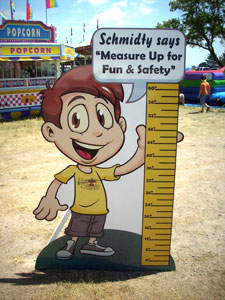
\includegraphics[width=\textwidth]{height}}
\end{minipage}
  \begin{minipage}{.65\linewidth}
Schmidty \cite{schmidt} has grown old and his vision is weak. He can no longer see if a person meets the height limit. The carnival organizers have installed a sensor to help. It beeps if any of the people in the waiting area is not eligible. Schmidty can move people in and out of the waiting area and then apply the sensor.

  \begin{parts}
  \part A family of 5 is trying to sneak in their toddler who does not meet the limit. Describe how Schmidty can identify the toddler in no more than 3 applications of the sensor.
  \part What is the smallest number of times that Schmidty needs to apply the sensor for a family of size $n$ in which only one person is below the limit. Justify your answer.
  \end{parts}
\end{minipage}
\begin{solution}
    % Enter your solution here.
     (a) There could be a post designed for maximum height of a person that is allowed to enter. A sensor should be fitted in the inside of that post (under the arch of the post). In this sensor the minimum value of height of the person allowed to enter should be preset. That sensor should first measure the length from the post to the ground, lets call it x cm and then measure the length from the post to the top of the persons head, lets call it y cm. After this it should calculate x-y and if it this value is less than the minimum value of the height preset in the sensor, the sensor should start beeping fast. Another second application of the sensor would be that it will have a ultrasound detection system which detects how many people are going through the sensor. The ultrasound will be transmitted by the sensor and if there are multiple people going through it, the sound will be reflected and the receiver will find out from the angle of the reflection that there is more than 1 person going through the sensor. As soon as it detects more than 1 person going through it will start beeping in another tone. 
    (b) It will need to apply the sensor only once in which it will first detect the number of people going through the sensor and then detect the height of the person when one person goes through it at a time.
  \end{solution}
\end{questions}

\begin{thebibliography}{9}
\bibitem{schmidt}
  TJ Schmidt \& Company (Standish, MI). \emph{Safety \& Maintenance}. \url{https://tjschmidtcarnival.com/pageserver/safety}. \textit{Last accessed on 6 Jan, 2023}.
\end{thebibliography}

\end{document}

%%% Local Variables:
%%% mode: latex
%%% TeX-master: t
%%% End:
